\subsection{Batch Normalization and Zero-mean Input}
\label{sec:appendix_batchnorm}
In this section, we show the results on networks with using Batch normalization (BN) \citep{ioffe2015batch}. For layers after BN, we have $\E[\vx]\approx 0$ so that $\E[\vx]\E[\vx]^\T$ no longer dominates $\mSigma_\vx$ and the low rank structure of $\E[\vx\vx^\T]$ should disappear. Thus, we can further expect that the overlap between top eigenspace of layer-wise Hessian among different models will not have a peak.

\tableref{tab:appendix_bn_xxT} shows the same experiments done in \tableref{tab:appendix_xxT_spec_fc}. The values for each network are the average of 3 different models. It is clear that the high inner product and large spectral ratio both do not hold here, except for the first layer where there is no normalization applied. Note that we had channel-wise normalization (zero-mean for each channel but not zero-mean for $\vx$) for conv1 in LeNet5 so that the spectral ratio is also small.
\begin{table}[ht]
\small
    \centering
    \caption{Structure of $\E[\vx\vx^\T]$ for BN networks}
    \vskip 0.1in
    \begin{center}
    \begin{small}
\begin{tabular}{llccccccc}
\toprule
        &              &       & \multicolumn{3}{c}{$(v_1^\T\hE[\vx])^2$} & \multicolumn{3}{c}{$\lambda_1/\lambda_2$} \\
Dataset & Network      & \# fc & mean        & min         & max         & mean         & min          & max         \\
\midrule
MNIST   & F-$200^2$-BN & 2     & 0.062       & 0.001       & 0.260       & 1.16         & 1.04         & 1.30        \\
        & F-$600^2$-BN & 2     & 0.026       & 0.000       & 0.063       & 1.13         & 1.02         & 1.26        \\
        & F-$600^4$-BN & 4     & 0.027       & 0.000       & 0.146       & 1.11         & 1.03         & 1.19        \\
        \midrule
CIFAR10 & LeNet5-BN & 3     & 0.210       & 0.001       & 0.803       & 1.54         & 1.20         & 1.89        \\
        \bottomrule
\end{tabular}
    \end{small}
    \end{center}
  \label{tab:appendix_bn_xxT}%
\end{table}

\figureref{fig:app_exp_bn_overlap}(a) shows that $\E[\vx\vx^\T]$ is no longer close to rank 1 when having BN. This is as expected. However, $\E[\vx\vx^\T]$ still has a few large eigenvalues.

\figureref{fig:app_exp_bn_overlap}(b) shows the eigenvector correspondence matrix of True Hessian with $\E[\vx\vx^\T]$ for fc1:LeNet5. Because $\E[\vx\vx^\T]$ is no longer close to rank 1, only very few eigenvectors of the layer-wise Hessian will have high correspondence with the top eigenvector of $\E[\vx\vx^\T]$, as expected. This directly leads to the disappearance of peak in top eigenspace overlap of different models, as shown in \figureref{fig:app_exp_bn_overlap}. The peak still exists in conv1 because BN is not applied to the input.

% \begin{figure}[th]
%     \centering
%     \vspace{-1em}
%     \subfigure[\small{Eigenspectrum of  $\E[\vx\vx^\T]$}]{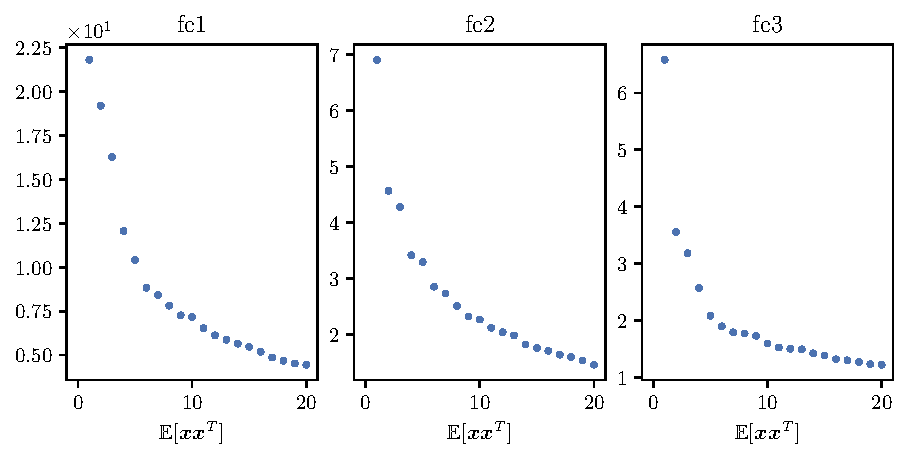
\includegraphics[width=0.48\linewidth]{Appendix_Figures/Explanation_LeNet5Case/BN/sigvals_xxt_t20_CIFAR10_Exp1_LeNet5_BN_nl_fixlr0.01R2_E-1.pdf}}
%     \subfigure[\small{True Hessian (fc1)}]{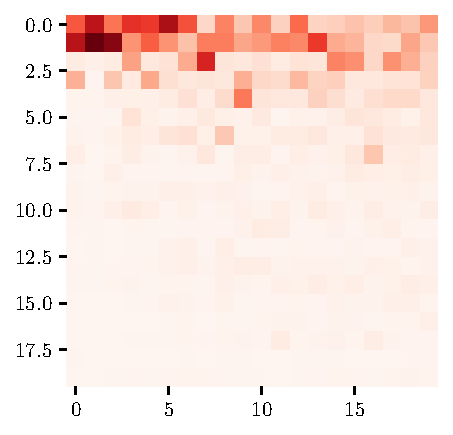
\includegraphics[width=0.24\linewidth]{Appendix_Figures/Explanation_LeNet5Case/BN/xxT_Trueest_real_corr_expand_t20_CIFAR10_Exp1_LeNet5_BN_nl_fixlr0.01R2_E-1_fc1.pdf}}
%     \subfigure[\small{Approx Hessian (fc1)}]{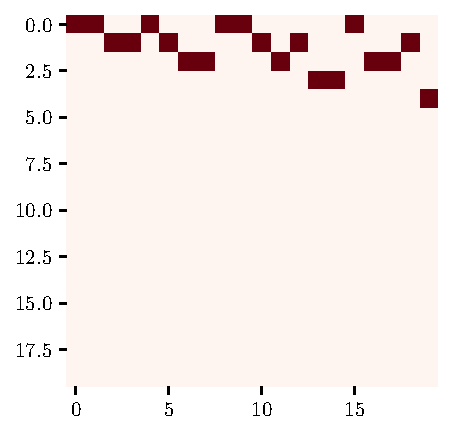
\includegraphics[width=0.24\linewidth]{Appendix_Figures/Explanation_LeNet5Case/BN/xxT_Approxest_real_corr_expand_t20_CIFAR10_Exp1_LeNet5_BN_nl_fixlr0.01R2_E-1_fc1.pdf}}
%     \caption{Eigenspectrum and Eigenvector correspondence matrices with $\E[\vx\vx^T]$ for LeNet5-BN.}
%     \label{fig:app_exp_bn_overlap}
% \end{figure}

\begin{figure}[ht]
    \centering
\begin{subfigure}[b]{0.5\textwidth}
    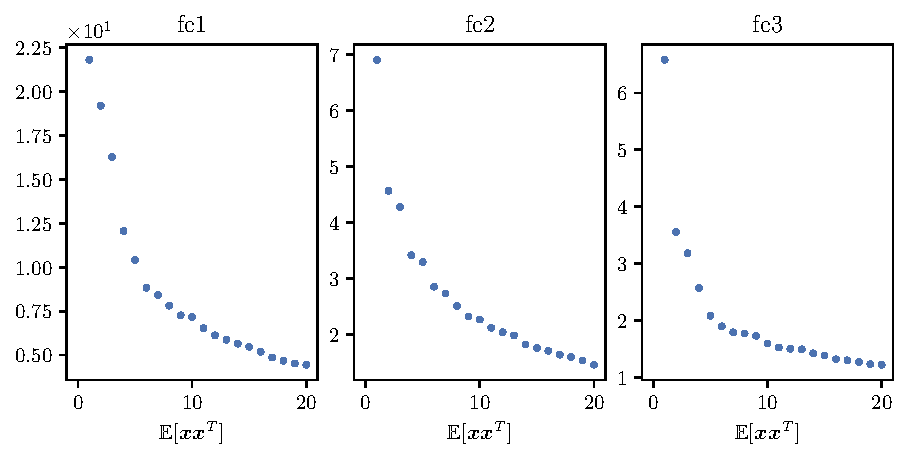
\includegraphics[width=\textwidth]{Appendix_Figures/Explanation_LeNet5Case/BN/sigvals_xxt_t20_CIFAR10_Exp1_LeNet5_BN_nl_fixlr0.01R2_E-1.pdf}
    \caption{Eigenspectrum for $\E[\vx\vx^\T]$}
    \label{fig:app_exp_bn_xxT_fc_eigenspec}
\end{subfigure}%
\begin{subfigure}[b]{0.25\textwidth}
    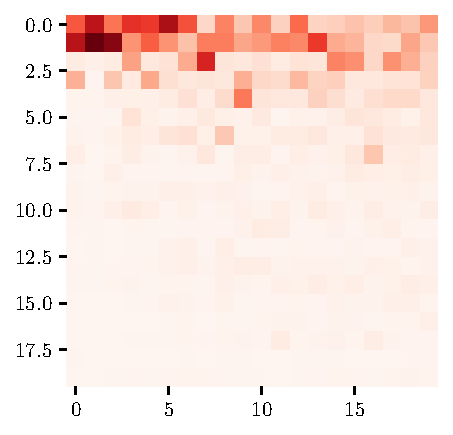
\includegraphics[width=\textwidth]{Appendix_Figures/Explanation_LeNet5Case/BN/xxT_Trueest_real_corr_expand_t20_CIFAR10_Exp1_LeNet5_BN_nl_fixlr0.01R2_E-1_fc1.pdf}
    \caption{True Hessian with\\ $\E[\vx\vx^\T]$ (fc1:LeNet5-BN)}
    \label{fig:app_exp_bn_corr_true}
\end{subfigure}%
\begin{subfigure}[b]{0.25\textwidth}
    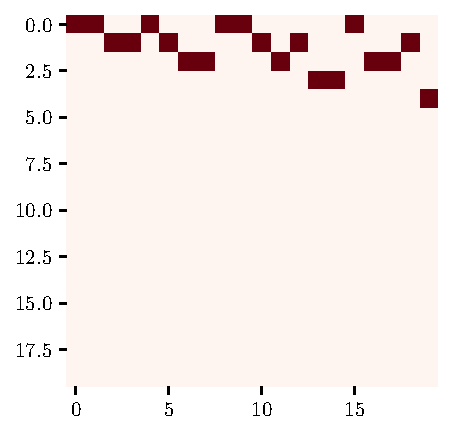
\includegraphics[width=\textwidth]{Appendix_Figures/Explanation_LeNet5Case/BN/xxT_Approxest_real_corr_expand_t20_CIFAR10_Exp1_LeNet5_BN_nl_fixlr0.01R2_E-1_fc1.pdf}
    \caption{Approx Hessian with\\ $\E[\vx\vx^\T]$ (fc1:LeNet5-BN)}
    \label{fig:app_exp_bn_corr_est}
\end{subfigure}
\label{fig:app_exp_bn_corr}
\caption{Eigenspectrum and Eigenvector correspondence matrices with $\E[\vx\vx^\T]$ for LeNet5-BN.}
\end{figure}
\begin{figure}[ht]
    \centering
    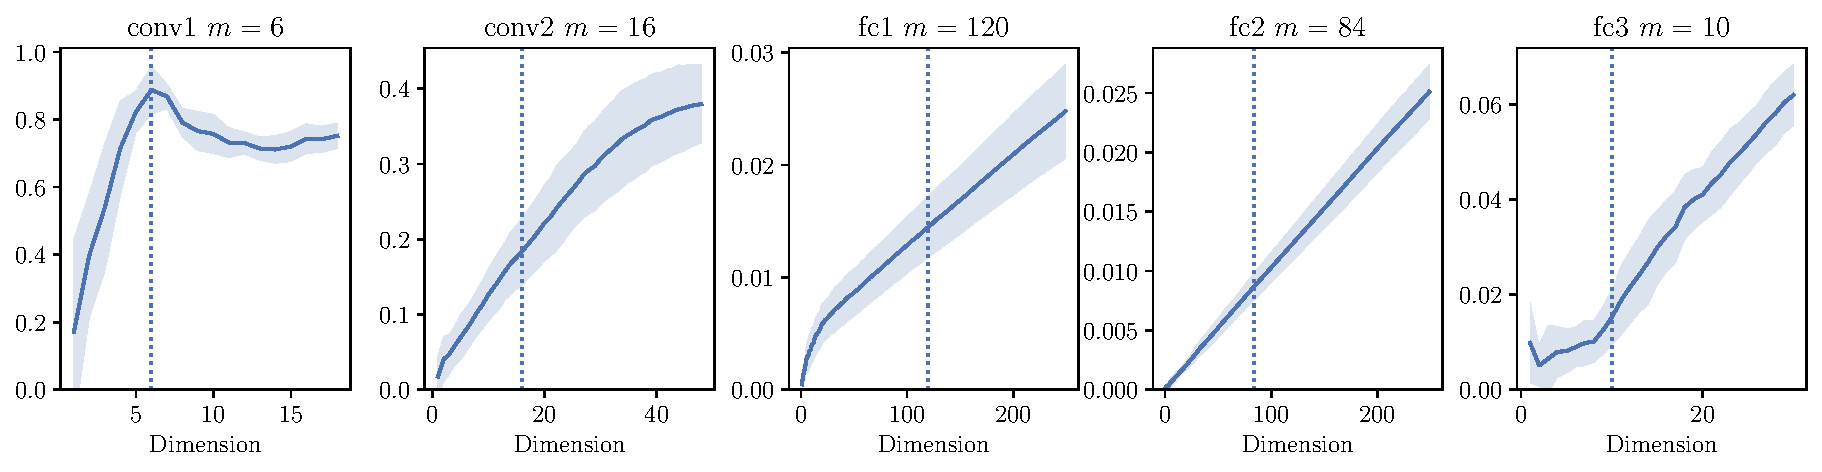
\includegraphics[width=\textwidth]{Appendix_Figures/Explanation_LeNet5Case/BN/DimOverlap_CIFAR10_LeNet5_BN_nl_fixlr0.01_appendix_full.pdf}
    \caption{Eigenspace overlap of different models of LeNet5-BN.}
    \label{fig:app_exp_bn_overlap}
\end{figure}

Comparing \figureref{fig:app_exp_bn_overlap}(b) and \figureref{fig:app_exp_bn_overlap}(c), we can see that the Kronecker factorization still gives a reasonable approximation for the eigenvector correspondence matrix with $\E[\vx\vx^\T]$, although worse than the cases without BN (\figureref{fig:Corr_fc}).

\begin{figure}[ht]
\centering
\begin{subfigure}[b]{0.35\textwidth}
        \captionsetup{justification=centering}
    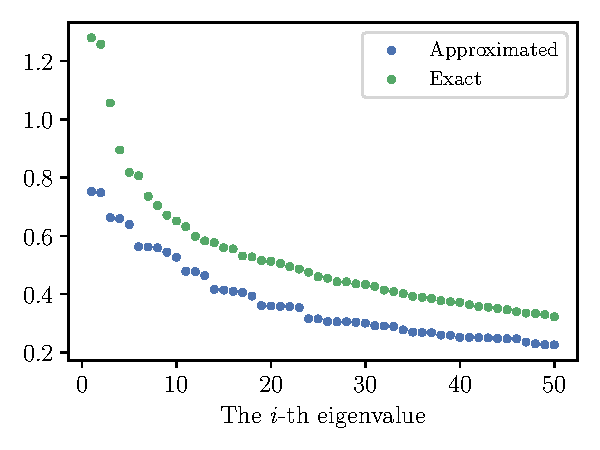
\includegraphics[width=\textwidth]{Appendix_Figures/Explanation_LeNet5Case/BN/eigenval_compare_top50_CIFAR10_Exp1_LeNet5_BN_nl_fixlr0.01R2_E-1_fc1.pdf}
    \caption{Top eigenvalues of approximated \\and exact layer-wise Hessian for fc2.}
    \label{fig:app_exp_bn_approx_eigenvalues}
\end{subfigure}%
\begin{subfigure}[b]{0.35\textwidth}
        \captionsetup{justification=centering}
    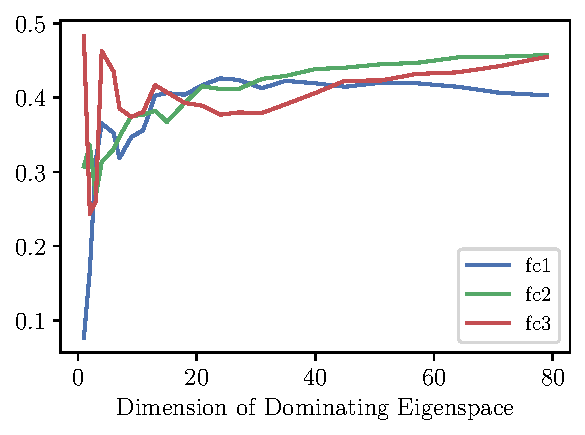
\includegraphics[width=\textwidth]{Appendix_Figures/Explanation_LeNet5Case/BN/sample_kron_decomp_traceoverlap_d80_CIFAR10_Exp1_LeNet5_BN_nl_fixlr0.01R2_E-1.pdf}
    \caption{Top eigenspace overlap between \\approximated and true layer-wise Hessian.}
    \label{fig:app_exp_bn_approx_overlap}
\end{subfigure}
\caption{Comparison between the true and approximated layer-wise Hessians for LeNet5-BN.}
\label{fig:app_exp_bn_approx}
\end{figure}
\figureref{fig:app_exp_bn_approx} compare the eigenvalues and top eigenspaces of the approximated Hessian and the true Hessian for LeNet5 with BN. The approximation using Kronecker factorization is also worse than the case without BN (\figureref{fig:eigeninfo_approx}). However, the approximation still gives meaningful information as the overlap of top eigenspace is still highly nontrivial.

% \begin{figure}[th]
%     \centering
%     \vspace{-1em}
%     \subfigure[\centering\small{Top eigenvalues of approximated \\and exact layer-wise Hessian for fc2.}]{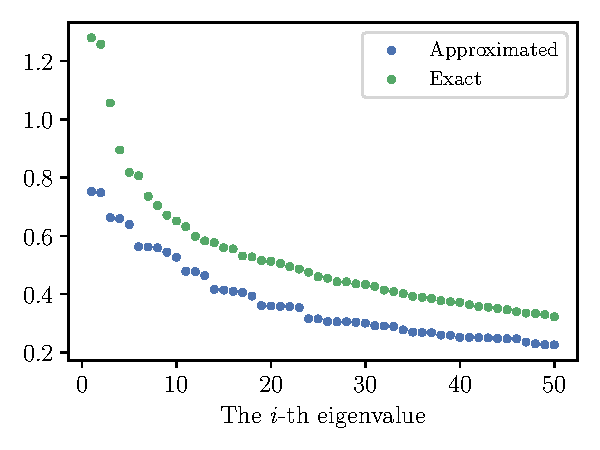
\includegraphics[width=0.48\linewidth]{Appendix_Figures/Explanation_LeNet5Case/BN/eigenval_compare_top50_CIFAR10_Exp1_LeNet5_BN_nl_fixlr0.01R2_E-1_fc1.pdf}}
%     \subfigure[\centering\small{Top eigenspace overlap between \\approximated and true layer-wise Hessian.}]{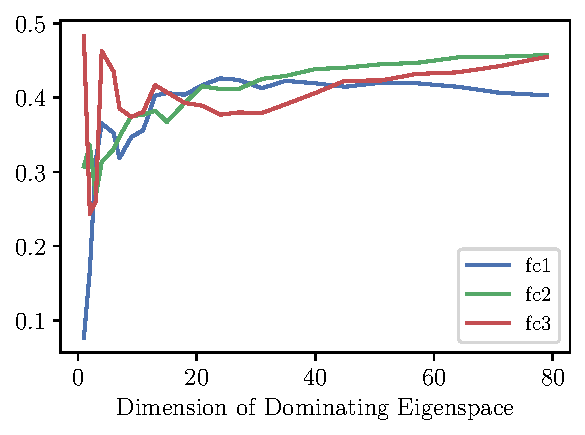
\includegraphics[width=0.48\linewidth]{Appendix_Figures/Explanation_LeNet5Case/BN/sample_kron_decomp_traceoverlap_d80_CIFAR10_Exp1_LeNet5_BN_nl_fixlr0.01R2_E-1.pdf}}
%     \caption{Comparison between the true and approximated layer-wise Hessians for LeNet5-BN.}
%     \label{fig:app_exp_bn_approx}
% \end{figure}